\section{Theoretical Framework}

This framework outlines sexual selection dynamics by combining deterministic and stochastic approaches. We first present Evolutionary Game Theory and stability analysis (Section \ref{sec:EGT} and \ref{sec:SA}) as deterministic foundations, then extend to finite populations using Markov chains, the master equation, and the Fokker--Planck approximation (Sections \ref{sec:Markov}--\ref{sec:fokker}). We discuss the Moran and Wright--Fisher processes as stochastic evolutionary models (Section \ref{sec:Moran}), introduce fitness-landscape parameters to characterize system behavior (Section \ref{sec:fitness}), link these ideas to sexual selection in guppies \textit{Poecilia reticulata} (Section \ref{sec:biology}), and finally examine realistic dynamics via nonlinear parameters (Section \ref{sec:nolinear}).\\ 


\subsection{Evolutionary Game Theory}
\label{sec:EGT}

Evolutionary Game Theory \textbf{(EGT)}, as a branch of game theory\footnote{
Game Theory rose formally in the 20th century. This teory consolidated a fundamental tool  for the analysis of individual strategies in competition contexts, where each individual depends on their actions and the actions of others among their group. Firstly, John von Neumann 1928 had expose about minimax theorem wich talks about of an optimal strategy in the sum of zero game. Then, John von Neumman and Oskar Morgenstern  published in 1944 the book \textit{Theory of Games and Economic Behavior}, which laid the foundations of game theory. Lastly, from 1950 onwards, other authors have been working  in go deeper into this subject as John Nash conceptualized the Nash equilibrium \cite{vonneumann1944, GameTheoryVery, nasar1998}.\\ 
}, initially applied for by John Maynard Smith and George Price  (\cite{maynardsmith1973, maynardsmith1982} explain in Nowak chapter 4  \cite{nowakEvolutionaryDynamicsExploring2006} and \cite{freyEvolutionaryGameTheory2010}). It is a form to simulate natural selection via the interplay between population and their strategies.
It is then a transition from classical rational players to evolutionary forces such as fitness, selection or
mutation. Acording to Frey \cite{freyEvolutionaryGameTheory2010} in a 
jornal as a theorical physics theory, EGT is a mathematical framework that studies the dynamics of
strategic interactions among populations of individuals where  noise have a significant role in the coexistence, evolution, and even extinction of species. In this project, we will focus on well-mixed population \footnote{According to Frey \cite{freyEvolutionaryGameTheory2010} well-mixed describes systems in which individuals move (or diffuse) so extensively that spatial degrees of freedom can be disregarded, and it can be assumed that every individual interacts with all others simultaneously. }.\\

Building on this framework, one can construct a game matrix for purposes of this project, as table \ref{tab:1}, based on two types of phenotypes: those that are sexually selected (A) and those that are not (B), considering predation as a factor of selective pressure. This matrix makes it possible to analyze the interactions between phenotypes and determine the optimal strategies for each. \\ 

\begin{table}[!h]
    \centering
    \begin{tabular}{c|cc}
        & Shoal A& Shoal B\\
        \hline
        Phenotype A & $W_{AA}$ & $W_{AB}$ \\
        Phenotype B & $W_{BA}$ & $W_{BB}$ \\
    \end{tabular}
    \caption{Game matrix for two phenotypes (A (Sexually Selected) and B (Non-Selected)) under sexual selection and predation. The elements $W_{ij}$  represent the payoffs obtained by each phenotype as a function of its interaction with the other.}
    \label{tab:payoffMatrix}
\end{table}



\subsection{Stability Analysis}
\label{sec:SA}
To describe deterministically how the phenotypic composition of the population changes over time, let \(p = \frac{i}{N}\) for a finite population, where \(i\) is the number of individuals of phenotypes \(A\). The dynamics of the frequency of phenotype \(A\) can then be modeled by the continuous-time replicator equation:

\begin{equation}
    \dot{p} = p(1-p)(\Pi_A - \Pi_B)
    \label{eq:p}
\end{equation}


Where 
\begin{equation}
    \Pi_A = p W_{AA} + (1-p) W_{AB}\ \quad  \text{and} \quad \Pi_B = p W_{BA} + (1-p) W_{BB}
    \label{eq:piA}
\end{equation}
\\

Here, \(W_{nm}\) denotes the payoff received by an individual of phenotype \(n\) when interacting with phenotype \(m\). Two additional quantities characterize the evolutionary dynamics are the mean population fitness and the fitness difference between phenotypes, defined respectively as

\begin{equation}
    \overline{\Pi}=p\Pi_A+(1-p)\Pi_B,
    \label{eq:meanPi}
\end{equation}

\begin{equation}
\Delta\Pi=\Pi_A-\Pi_B,
\label{eq:diffPi}
\end{equation}

capture the relative selective advantage of phenotype \(A\) over phenotype \(B\). A positive fitness difference promotes an increase in the frequency of phenotype \(A\), whereas a negative difference favors phenotype \(B\). These quantities therefore provide the basis for identifying evolutionary equilibria and assessing their stability under the replicator dynamics. \\

The equilibria follow from setting \(\dot{p}=0\), and their stability is determined by examining the direction of the evolutionary dynamics near each equilibrium. Depending on the relative fitness values, the system displays four evolutionary regimes in the generic case of strict fitness inequalities, together with the special case of complete neutrality.\\ 

\begin{itemize}
    \item \textbf{A dominates B:} Occurs if \(W_{AA} > W_{BA}\) and \(W_{AB} > W_{BB}\). Phenotype \(A\) always has a higher fitness regardless of the shoal composition, driving the system to the \(p=1\) attractor.\\
  
    \item \textbf{B dominates A:} Occurs if \(W_{AA} < W_{BA}\) and \(W_{AB} < W_{BB}\). The system converges to \(p=0\).\\

    \item \textbf{Bi-stability:} Occurs if \(W_{AA} > W_{BA}\) and \(W_{BB} > W_{AB}\). There are two stable attractors (\(p=0\) and \(p=1\)) separated by an unstable interior equilibrium.\\
    
    \item \textbf{Stable Coexistence:} Occurs if \(W_{AA} < W_{BA}\) and \(W_{BB} < W_{AB}\). The system converges to an interior equilibrium 
    \begin{equation}
        p^* = \frac{W_{BB}-W_{AB}}{W_{AA}-W_{AB}-W_{BA}+W_{BB}}
        \label{eq:pEquilibrium}
    \end{equation}

    where both phenotypes coexist.\\
    
    \item \textbf{Neutrality:} Occurs when \(W_{AA}=W_{BA}\) and \(W_{AB}=W_{BB}\). Both phenotypes have identical fitness for any population composition, resulting in \(\dot{p}=0\) for all \(p\). In finite populations, however, stochastic genetic drift may still produce changes in phenotype frequencies.
\end{itemize}

While the replicator equation characterizes the temporal evolution of phenotype frequencies and the stability of population equilibria, evolutionary stability provides a complementary criterion based on resistance to invasion by rare mutants. This distinction is captured by the concept of an  \textbf{Evolutionarily Stable Strategy (ESS)}, which identifies strategies that cannot be successfully invaded by an initially rare alternative strategy under the assumptions of the evolutionary game according to \cite{mit2021game} and \cite{nowakEvolutionaryDynamicsExploring2006}. For phenotype \(A\) to be an ESS, it must satisfy either:

\begin{itemize}
    \item \textbf{Strict Nash Equilibrium:} \(W_{AA} > W_{BA}\) (A is strictly better than B when playing against A). \\ 
    
    \item \textbf{Weak Nash Equilibrium:} If \(W_{AA} = W_{BA}\), then it must hold that \(W_{AB} > W_{BB}\) (A is better than B when playing against B).
\end{itemize}

\vspace{1em}

\subsection{Markov Chains}
\label{sec:Markov}

 To incorporate the stochastic fluctuations in finite, evolutionary dynamics can be modeled as a discrete-time Markov chain, where changes in population composition are governed by probabilistic transitions between discrete states.

\begin{figure}[h!]
    \centering
    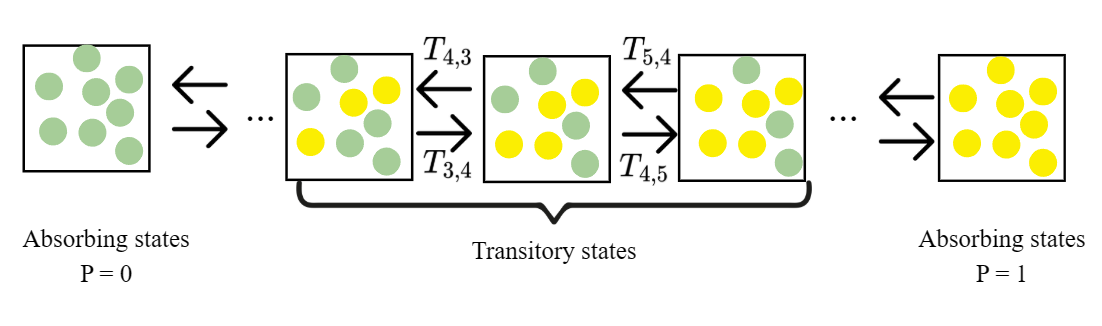
\includegraphics[width=1\linewidth]{Imagenes/Markov Chains.png}
    \caption{Representation of a finite-population Markov chain describing the stochastic evolution of two competing phenotypes A (yellow) and  B (green). Each state represents a population composition, with transitions between neighboring states governed by the probabilities \(T_{i,j}\). The intermediate states are transient, allowing fluctuations in phenotype frequencies, whereas the boundary states \(p=0\) and \(p=1\) are absorbing, corresponding to the fixation of one phenotype and the extinction of the other, inspired by \cite{nowakEvolutionaryDynamicsExploring2006}.}
    \label{fig:markovChains}
\end{figure}    

\clearpage 

Therefore the probability of transitions \(T_{i,j}\) based in the process of Liu et al \cite{liuFixationProbabilitiesEvolutionary2015}, using equations \eqref{eq:piA}, are: 

\begin{equation}
    T_{i,i+1}=  \frac{i \cdot \Pi_A}{i \cdot \Pi_A + (N-i)\cdot \Pi_B}\frac{N-i}{N}
    \label{eq:transicionmas}
\end{equation}

\begin{equation}
    T_{i,i-1}=  \frac{(N-i) \cdot \Pi_B}{i \cdot \Pi_A + (N-i)\cdot \Pi_B}\frac{i}{N}
    \label{eq:transicionmenos}
\end{equation}

\begin{equation}
    T_{i,i}=  1-T_{i,i+1} - T_{i,i-1}
    \label{eq:sintransicion}
\end{equation}

In the absence of mutations, the states \(p=0\) and \(p=1\) are absorbing, corresponding to the extinction and fixation of phenotype \(A\), respectively. The remaining states are transient, allowing stochastic changes in population composition until one of the absorbing states is reached. The process is described in the figure \ref{fig:markovChains}; it is based on birth-death process, specifically in Moran process, it will be described after.\\  

The transition probabilities define a tridiagonal matrix \(M\) of dimensions \((N+1)\times(N+1)\), since the number of individuals exhibiting phenotype A can increase or decrease by at most one during each transition. Each state \(i\in\{0,1,\ldots,N\}\) represents the number of individuals of phenotype A, while the matrix elements \(M_{ij}\) describe the probability of transitioning from state \(i\) to state \(j\). In the absence of mutation, the boundary states \(i=0\) and \(i=N\) are absorbing, corresponding to the fixation of phenotypes B and A, respectively. The transition matrix is therefore expressed as

\begin{equation}
M=
\begin{pmatrix}
1 & 0 & 0 & \cdots & 0 & 0 \\
T_{1,0} & T_{1,1} & T_{1,2} & \cdots & 0 & 0 \\
0 & T_{2,1} & T_{2,2} & \ddots & 0 & 0 \\
\vdots & \ddots & \ddots & \ddots & \ddots & \vdots \\
0 & 0 & \cdots & T_{N-1,N-2} & T_{N-1,N-1} & T_{N-1,N} \\
0 & 0 & \cdots & 0 & 0 & 1
\end{pmatrix}.
\label{eq:moran_transition_matrix}
\end{equation}

For each interior state \(1\leq i\leq N-1\), the transition probabilities satisfy

\begin{equation}
T_{i,i-1}+T_{i,i}+T_{i,i+1}=1.
\end{equation}

The evolution of the population probability distribution is then determined by successive applications of the transition matrix:

\begin{equation}
\mathbf{x}^{(n)}=\mathbf{x}^{(0)}M^n,
\label{eq:markov_evolution}
\end{equation}

where \(\mathbf{x}^{(0)}\) is the initial probability distribution over the population states and \(n\) denotes the number of Markov chain steps.
\clearpage

\subsection{Master Equation}
\label{sec:master}

While the transition probabilities characterize the possible changes in population composition during a single reproduction--replacement event, they do not explicitly describe how the probability distribution over population states evolves over time. This evolution is described by the master equation, which follows from the Markov property and accounts for probability flows between neighboring states. \\ 

Let \(P_i(n)\) denote the probability of finding exactly \(i\) individuals exhibiting phenotype A after \(n\) steps of the Markov chain. For the discrete-time birth--death process considered here, the probability distribution evolves according to

\begin{equation}
    P_i(n+1)
    =
    P_{i-1}(n)T_{i-1,i}
    +
    P_i(n)T_{i,i}
    +
    P_{i+1}(n)T_{i+1,i},
    \label{eq:probDynamics}
\end{equation}

where the three terms represent the probabilities of entering state \(i\) from state \(i-1\), remaining in state \(i\), and entering from state \(i+1\), respectively.\\ 

Equivalently, the master equation can be expressed in terms of the net probability flow between neighboring states:

\begin{equation}
\begin{aligned}
    P_i(n+1)-P_i(n)
    ={}&
    P_{i-1}(n)T_{i-1,i}\\
    &+P_{i+1}(n)T_{i+1,i}\\
    &-P_i(n)\left(T_{i,i+1}+T_{i,i-1}\right).
\end{aligned}
\label{eq:Nose}
\end{equation}

Both expressions apply to the interior states \(1\leq i\leq N-1\). In the absence of mutation, the boundary states \(i=0\) and \(i=N\) are absorbing, corresponding to the fixation of phenotypes B and A, respectively. Their probabilities evolve according to

\begin{equation}
\begin{aligned}
P_0(n+1)&=P_0(n)+P_1(n)T_{1,0},\\
P_N(n+1)&=P_N(n)+P_{N-1}(n)T_{N-1,N}.
\end{aligned}
\label{eq:master_boundaries}
\end{equation}

The master equation can also be written in matrix form as

\begin{equation}
\mathbf{x}^{(n+1)}=\mathbf{x}^{(n)}M,
\label{eq:master_matrix}
\end{equation}

where \(\mathbf{x}^{(n)}\) is the probability distribution over all population states and \(M\) is the transition matrix of the Markov chain. \\ 

This formulation provides a probabilistic description of evolutionary dynamics in finite populations, incorporating both directional selection and demographic fluctuations. Unlike the deterministic replicator equation, it describes the redistribution of probability across population states and allows the temporal evolution of fixation probabilities to be investigated.


\clearpage 


\subsection{Fokker-Planck Continuous Approximation}
\label{sec:fokker}
For sufficiently large populations, a continuous
approximation can be introduced to describe the stochastic
evolution of phenotype frequencies. To obtain this approximation, we define the frequency of
phenotype  \(A\), such that changes between
neighboring states correspond to increments of
\(\Delta p=1/N\). We also introduce the rescaled time
\(\tau=t/N\) and the continuous probability density
\(P(p,\tau)\approx NP_i(t)\). \\ 

Assuming sufficiently smooth transition probabilities
and probability densities, a second-order Kramers--Moyal, as described by Moyal in \cite{moyalStochasticProcessesStatistic1949},
expansion of the master equation yields the
Fokker--Planck approximation: 


\begin{equation}
    \frac{\partial P(p,\tau)}{\partial \tau}
    =
    -\frac{\partial}{\partial p}
    \left[A(p)P(p,\tau)\right]
    +
    \frac{1}{2}
    \frac{\partial^2}{\partial p^2}
    \left[B(p)P(p,\tau)\right].
    \label{eq:FokkerPlanck}
\end{equation}

Here, \(A(p)\) and \(B(p)\) are the drift and diffusion
coefficients, respectively, defined in terms of the
transition probabilities as: 

\begin{equation}
    A(p)=T_{i,i+1}-T_{i,i-1}, \quad   B(p)=\frac{T_{i,i+1}+T_{i,i-1}}{N}, 
    \label{eq:driftCoefficient}
\end{equation}

where the transition probabilities are evaluated at \(i=Np\).Substituting the transition probabilities previouslydefined for the Moran process, the drift coefficient
becomes and the diffusion coefficient is given by, respectively

\begin{equation}
    A(p)=
    \frac{
        p(1-p)(\Pi_A-\Pi_B)
    }{
        p\Pi_A+(1-p)\Pi_B
    }, \quad  B(p)=
    \frac{
        p(1-p)(\Pi_A+\Pi_B)
    }{
        N[p\Pi_A+(1-p)\Pi_B]
    }.
    \label{eq:driftFitness}
\end{equation}

The drift coefficient describes the directional
change in phenotype frequency associated with fitness
differences, while the diffusion coefficient quantifies
the stochastic fluctuations arising from finite
population size.\\ 

In particular, the diffusion coefficient scales
inversely with \(N\), indicating that stochastic
fluctuations become weaker as the population grows.
The resulting Fokker--Planck equation therefore
provides a continuous approximation connecting
stochastic birth--death dynamics with the deterministic
evolutionary framework.


\subsection{Moran Process}
\label{sec:Moran}

This algorithm is a dynamical simulation of a birth-death process (it keeps the population constant), in which an individual from a population is randomly selected to reproduce, with a probability weighted by its fitness. Then, another individual is randomly selected to die and be replaced by the offspring of the first selected individual, as described in figure \ref{fig:moranProcess}. This process is repeated iteratively at each step of the simulation, allowing observation of how the population of a given phenotype spreads or vanishes over time. The probability of fixation of a phenotype depends on its relative fitness and on the composition of the phenotypes, which makes the Moran process a useful tool for studying the evolution of phenotypes under different selective conditions. This process was originally described by Moran \cite{moran1958}, as noted by Galanis et al. \cite{galanisAmplifiersMoranProcess2017} and in Chapter 6 of Nowak \cite{nowakEvolutionaryDynamicsExploring2006}. \\ 


\begin{figure}[h!]
    \centering
    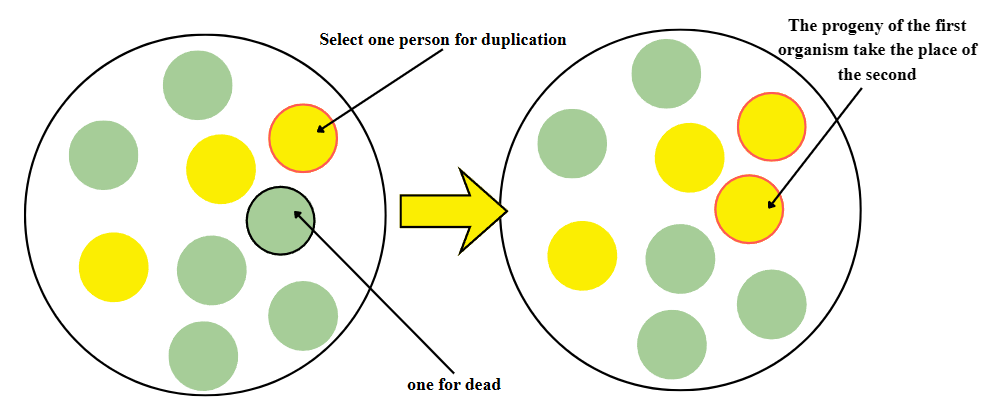
\includegraphics[width=0.9\linewidth]{Imagenes/Moran Process.png}
    \caption{Schematic representation of the Moran process. At each step, in a finite population of $N$ individuals, an individual is selected for reproduction (duplication) with a probability proportional to its fitness (upper arrow), while another is chosen at random to die (lower arrow). The offspring of the first replaces the second, keeping the population size constant. This iterative process allows observation of how phenotypes spread or go extinct over time inspired by \cite{nowakEvolutionaryDynamicsExploring2006}.}
    \label{fig:moranProcess}
\end{figure}


A second type of birth-death process is the Wright–Fisher process, which, like the Moran process, assumes a finite population of constant size \(N\) but differs in its reproductive scheme. In the Wright–Fisher process assumes discrete, non-overlapping generations: all individuals reproduce simultaneously, each contributing offspring to a common pool in proportion to its payoff (fitness), and the next generation is then sampled randomly from this pool—formally, through \(N\). This results in a complete generational turnover at each step, rather than the single-individual replacement of the Moran process 
\cite{imhofEvolutionaryGameDynamics2006}. The Markov chain produced has two absorbing states identical to the original, but given the nearly all differential one-step transitions, it necessitates a different analytical approach. In conclusion, the use of the Moran process is explained by the fact that the Wright–Fisher process would be analytically more complicated than needed for the information the Moran approach provides.  \\ 



\subsection{Fitness Landscape}
\label{sec:fitness}
Originally introduced by Sewall Wright, the fitness landscape visualizes how biological configurations relate to evolutionary fitness; traditionally, it maps fitness across a multidimensional genetic space, revealing peaks, valleys, and regions of differing reproductive success \cite{nowakEvolutionaryDynamicsExploring2006,mccandlishVISUALIZINGFITNESSLANDSCAPES2011}. Here, we adapt this concept to a population of two competing phenotypes, representing the resulting landscape as a three-dimensional surface figure \ref{fig:fitnessLandscape}. Although peaks and valleys denote higher and lower fitness, their correspondence with evolutionary attractors or unstable equilibria must be established through the population dynamics.


\begin{figure}[h!]
    \centering
    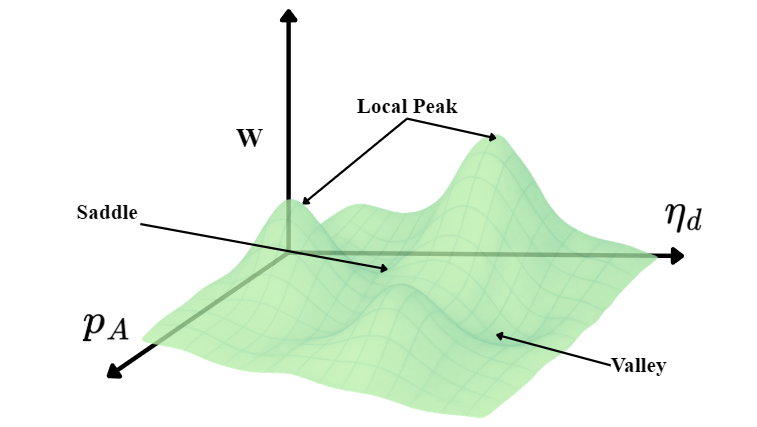
\includegraphics[width=0.75\linewidth]{Imagenes/Fitness Landscape.png}
    \caption{ Three-dimensional fitness landscape showing fitness \(W\)as a function of the initial density of phenotype A \(P_A\) and predator density \(\eta_d\), illustrating key topological features such as local peaks, valleys, and saddle points inspired by \cite{nowakEvolutionaryDynamicsExploring2006} .}
    \label{fig:fitnessLandscape}
\end{figure}

For the two-phenotype system, the fitness landscape can be built from the expected fitness of each phenotype, with the mean population fitness and the fitness difference defined in equations \ref{eq:meanPi} and\ref{eq:diffPi}. Both quantities can be visualized as surfaces, although the fitness difference conveys the direction of selection rather than absolute reproductive success.\\ 


In stochastic simulations, the mean change over a finite interval of \(x\) Moran steps can be estimated by averaging the slopes of \(R\) independent trajectories initialized at the same population composition:

\begin{equation}
\widehat{v}_x(p_0,\eta_d)
=
\frac{1}{R}
\sum_{r=1}^{R}
\frac{p_r(x)-p_0}{x},
\end{equation}

where \(p_r(x)\) is the proportion of phenotype \(A\) after \(x\) steps in realization \(r\). Evaluating this quantity across initial frequencies \(p_0\) and predation intensities \(\eta_d\) yields a three-dimensional surface representing a finite-time drift landscape, which characterizes the direction and magnitude of the mean evolutionary change. \\ 

From a physical perspective, evolutionary drift provides a useful analogy with a force field, as it describes the expected direction and magnitude of changes in population composition. In a one-dimensional evolutionary state space, an effective potential can be formally constructed by integrating the negative instantaneous drift with respect to the phenotypic frequency. However, this potential must be distinguished from mean population fitness, whose gradient does not generally determine the evolutionary dynamics. Furthermore, the drift field alone does not fully characterize stochastic evolution, since demographic fluctuations also contribute to the redistribution of probability across population states. This distinction motivates the complementary use of fitness landscapes, evolutionary drift, and stochastic population models.\\ 

\clearpage


\subsection{Biological Dynamics for Sexual Selection Poblation}
\label{sec:biology}

\begin{wrapfigure}{l}{0.5\textwidth}
    \centering
    \vspace{-1em}
    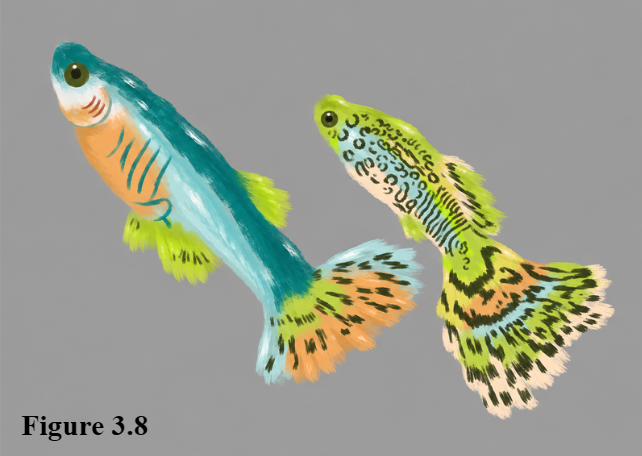
\includegraphics[width=\linewidth]{Imagenes/Guppies.png}
    \label{fig:guppiesdisform}
    \vspace{-2em}
\end{wrapfigure}

Although the theoretical framework developed in this study does not require a specific biological species, male guppies (\textit{Poecilia reticulata}) provide a suitable reference system due to the extensive experimental literature on sexual selection and predation. Guppies exhibit pronounced sexual dimorphism, with males displaying more conspicuous colour patterns than females, as illustrated in Figure \ref{fig:guppiesdisform}. Male reproductive success is strongly influenced by female mate choice and sexual attractiveness, consistent with the theory of secondary sexual traits \cite{andersson1994,houdeSexColorMate1997}. In particular, Houde \cite{houdeMATECHOICEBASED1987} demonstrated that female guppies preferentially associate and mate with males exhibiting larger areas of orange pigmentation, while Zahavi's handicap principle suggests that costly ornamentation may serve as a signal of individual quality \cite{zahavi1987signal}. However, these sexually attractive traits may also increase vulnerability to predators, generating opposing selective pressures. Godin and McDonough \cite{godinPredatorPreferenceBrightly2003} experimentally demonstrated that predatory cichlids preferentially attacked and captured more brightly coloured males, while female mating preferences and male reproductive behaviour may change in response to predation risk \cite{godinFemaleMateChoice1996,magnhagen1991}. Furthermore, the effectiveness and survival costs of visual signals depend on environmental conditions and their perception by potential mates and predators \cite{endler1991}. Predation pressure may also influence courtship displays, alternative mating tactics, and reproductive risk-taking behaviour \cite{bothamRISKSENSITIVEANTIPREDATORBEHAVIOR2008,smithBehavioralTypesPredictors2010,goslinePredatorinducedPlasticityGuppy2008}. Endler \cite{endlerNATURALSELECTIONCOLOR1980} demonstrated that predation regimes can shape the evolution of male coloration, with reduced predation generally favouring greater ornamentation and stronger predation favouring less conspicuous phenotypes. These observations illustrate the trade-off between reproductive attractiveness and predation-related survival costs, making guppies a biologically motivated reference system for investigating the evolutionary dynamics of alternative male phenotypes.\\ 

From a biological perspective, frequency dependence may arise from changes in predation vulnerability associated with the phenotypic composition of a shoal. Conspicuous individuals exhibit highly visible traits, such as bright coloration, whereas cryptic individuals display traits that reduce their detectability against the surrounding environment. Consequently, predominantly conspicuous groups may attract greater predator attention than cryptic groups. However, individual predation risk also depends on group composition: the \textit{oddity effect} may increase the vulnerability of individuals whose appearance differs from that of other group members, while the \textit{confusion effect} may reduce a predator's ability to identify and capture a particular individual within a group \cite{rodgersMixedphenotypeGroupingInteraction2013}. Although these mechanisms may operate asymmetrically, their opposing contributions are assumed to approximately compensate under the reference conditions considered, without implying universal cancellation. These biological mechanisms suggest that the fitness of each phenotype may depend not only on predation intensity and reproductive advantages, but also on the phenotypic composition of the population. This motivates the introduction of frequency-dependent
interactions in the evolutionary game-theoretic model.\\ 


\subsection{Nonlinear Parameters in Evolutionary Game Theory}
\label{sec:nolinear}

In classical evolutionary game theory \textbf{(EGT)}, payoff matrices generally contain constant entries, leading to expected fitness functions that depend linearly on population frequencies. However, this approximation may be insufficient for ecological systems in which the costs and benefits of interactions vary with population composition or the frequency of competing phenotypes. More general formulations allow the payoff matrix itself to depend on the evolutionary state of the population, introducing additional nonlinearities into the fitness functions \cite{broomNonlinearMultiplayerEvolutionary2016}. In this case, the payoff matrix becomes frequency-dependent, \(W=W(p)\), and the expected fitness functions are expressed as 

\begin{equation}
\begin{aligned}
\Pi_A(p) &= pW_{AA}(p)+(1-p)W_{AB}(p),\\
\Pi_B(p) &= pW_{BA}(p)+(1-p)W_{BB}(p).
\end{aligned}
\end{equation}

Consequently, the fitness difference \(\Delta\Pi(p)=\Pi_A(p)-\Pi_B(p)\) is generally nonlinear. Although the replicator equation retains its original structure,

\begin{equation}
\dot p=p(1-p)\Delta\Pi(p),
\end{equation}

the location and stability of evolutionary equilibria may change. The boundary equilibria \(p=0\) and \(p=1\) remain stationary, whereas interior equilibria satisfy \(\Delta\Pi(p^*)=0\)  , with \(0<p^*<1\). Their local stability is determined by

\begin{equation}
\left.\frac{d\dot p}{dp}\right|_{p=p^*}
=
p^*(1-p^*)
\left.\frac{d\Delta\Pi}{dp}\right|_{p=p^*}.
\label{eq:estabilidad}
\end{equation}

Thus, a negative derivative of the fitness difference indicates local asymptotic stability, while a positive derivative indicates instability. Similarly, \(p=0\) is locally asymptotically stable when \(\Delta\Pi(0)<0\), and \(p=1\) is locally asymptotically stable when \(\Delta\Pi(1)>0\). Equality cases require further analysis. Importantly, the mathematical frameworks of Markov chains, the master equation, and the Fokker--Planck approximation remain applicable without changes to their general structure. However, the transition probabilities and the corresponding drift and diffusion coefficients must be evaluated using the frequency-dependent fitness functions. \\ 


